\section{Introduction}

Ce chapitre présente le contexte général et la planification de notre projet de développement d'une \textbf{plateforme de gestion de projets (SGP)}. Nous y détaillerons la méthodologie adoptée, le cycle de vie du projet, et l'organisation du travail selon l'approche Scrum.

\section{Contexte général}

\subsection{Situation actuelle et pratique existante}

Les activités projet étaient pilotées avec des outils épars (tableurs, e-mails) sans référentiel unique ni workflow tracé. L'absence de backlog consolidé, de sprints synchronisés et de suivi quotidien des tâches compliquait la planification, la coordination inter-rôles et la prise de décision.

\textbf{Lacunes identifiées dans l'ancien processus :}
\begin{itemize}
    \item \textbf{Fragmentation des outils :} Utilisation dispersée de tableurs Excel, e-mails et documents Word sans intégration, créant des silos d'information et des risques de perte de données.
    \item \textbf{Absence de traçabilité :} Impossibilité de suivre l'évolution d'une demande client jusqu'au livrable final, compliquant la justification des choix et la validation avec les clients.
    \item \textbf{Planification hétérogène :} Chaque équipe utilisait ses propres méthodes de planification des sprints et jalons, rendant impossible une vue d'ensemble cohérente du portefeuille.
    \item \textbf{Application inégale des rôles :} Les responsabilités des différents acteurs (PO, SM, Dev, etc.) n'étaient pas clairement définies ni respectées de manière uniforme.
    \item \textbf{Indicateurs insuffisants :} Manque d'indicateurs fiables sur l'avancement, la vélocité des équipes et la charge de travail, empêchant un pilotage efficace.
    \item \textbf{Notifications manuelles :} Absence d'automatisation des notifications, créant des retards dans la communication et les prises de décision.
    \item \textbf{Gestion des changements chaotique :} Aucun processus structuré pour analyser l'impact des changements sur les coûts, délais et ressources.
\end{itemize}

\subsection{Objectif de la solution}

L'objectif principal est de fournir une \textbf{SGP unifiée} qui centralise et standardise l'ensemble des processus de gestion de projets. Cette plateforme doit permettre la \textbf{capture structurée des demandes client} avec un workflow de validation par la Direction, incluant la collecte d'informations détaillées, l'évaluation de la faisabilité technique et commerciale, et la prise de décision éclairée sur l'opportunité de contractualiser.

La solution doit également supporter la \textbf{création et le paramétrage complet d'un projet}, incluant la définition des phases de développement, l'établissement des jalons de validation, l'allocation des ressources humaines et matérielles, et la configuration des règles métier spécifiques au projet.

L'\textbf{exécution Scrum} constitue le cœur de la plateforme, avec la gestion du backlog priorisé par le Product Owner, la planification et l'exécution des sprints par le Scrum Master, la décomposition en user stories détaillées, et le suivi des tâches opérationnelles par les équipes de développement.

\section{Enjeux et objectifs}

Les enjeux majeurs du \textbf{SGP} sont: \textbf{visibilité portefeuille}, \textbf{pilotage par la valeur}, \textbf{réduction du temps de cycle} et \textbf{maîtrise des risques et des changements}. Ces enjeux se traduisent par les objectifs concrets suivants:

\begin{itemize}
    \item \textbf{Centralisation des artefacts} du projet: \texttt{Projet, Phase, Sprint, UserStory, Tache, Jalon, Backlog, Livrable, Validation, Changement}.
    \item \textbf{Exécution agile outillée}: priorisation du backlog par le PO, planification/démarrage de sprints par le SM, tableaux Kanban et mises à jour de tâches par Dev/QA.
    \item \textbf{Gouvernance et conformité}: jalons, validations de livrables, gestion des changements avec traçabilité.
    \item \textbf{Rôles et accès} robustes (JWT/OAuth2 Microsoft), gardes côté Angular et contrôles côté Spring Security.
    \item \textbf{Indicateurs temps réel}: KPI par projet/sprint (vélocité, avancement, charge, qualité), notifications WebSocket, analytics et exports via Power BI.
    \item \textbf{Référentiel amont}: intégration des demandes clients (\texttt{ClientInquiry}) et des contrats, menant à la création de projets.
\end{itemize}

\section{Méthodologie adoptée}

Pour ce projet, nous avons opté pour la \textbf{méthodologie Scrum}, qui favorise un développement itératif et incrémental à travers des sprints. Chaque sprint est planifié sur une durée de deux semaines, permettant de livrer des fonctionnalités prêtes à l'usage tout en recueillant régulièrement des retours des parties prenantes.

\subsection{Le cycle de vie du projet}

Le cycle de vie de notre projet comprend les activités suivantes :

\begin{enumerate}
    \item \textbf{Analyse des besoins et faisabilité :} Identification, recueil et formalisation des besoins fonctionnels et non fonctionnels, ainsi que des contraintes techniques et organisationnelles.
    \item \textbf{Planification et priorisation :} Création du backlog produit, définition des priorités et planification des tâches pour chaque sprint.
    \item \textbf{Conception :} Élaboration des spécifications générales et détaillées de l'architecture logicielle, des bases de données et des interfaces utilisateur.
    \item \textbf{Développement :} Implémentation progressive des fonctionnalités prévues dans les sprints, avec des revues de code et une intégration continue.
    \item \textbf{Tests :} Vérification de chaque fonctionnalité par des tests unitaires, fonctionnels et d'intégration pour garantir leur conformité aux spécifications.
    \item \textbf{Documentation :} Rédaction des informations nécessaires à l'utilisation, la maintenance et les futures évolutions du logiciel.
    \item \textbf{Livraison et déploiement :} Livraison progressive des incréments et mise en production du produit final.
\end{enumerate}

Cette approche agile assure une meilleure collaboration entre les parties prenantes et une flexibilité accrue face aux changements, tout en maintenant un haut niveau de qualité.

% --- Image de la méthodologie SCRUM ---
\begin{figure}[H] 
    \centering
    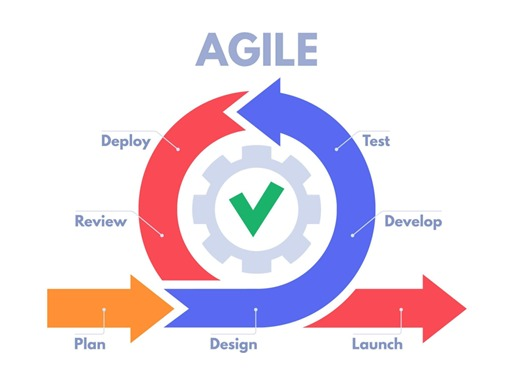
\includegraphics[width=1\textwidth]{Figures/Model_SCRUM.jpg}
    \caption{Modèle de la méthodologie SCRUM}
    \label{fig:methodo_scrum}
\end{figure}

\subsection{Modèle de travail}

Un projet logiciel doit suivre différentes phases jalonnées par des points de contrôle clés afin de garantir sa gestion dans un contexte de qualité. Chaque étape est associée à des livrables spécifiques validés en fonction des objectifs définis. Cette approche permet de maîtriser la conformité des livrables aux besoins exprimés, tout en s'assurant du respect des contraintes de coûts et de délais.

Parmi les modèles de développement logiciel, nous avons adopté une approche itérative basée sur la méthodologie Scrum. Contrairement au modèle en cascade, cette méthode repose sur des cycles itératifs (sprints) qui favorisent l'adaptation continue aux besoins évolutifs du projet. Chaque sprint se termine par la production d'un incrément fonctionnel validé par les parties prenantes.

% --- Image du modèle AGILE ---
\begin{figure}[H] 
    \centering
    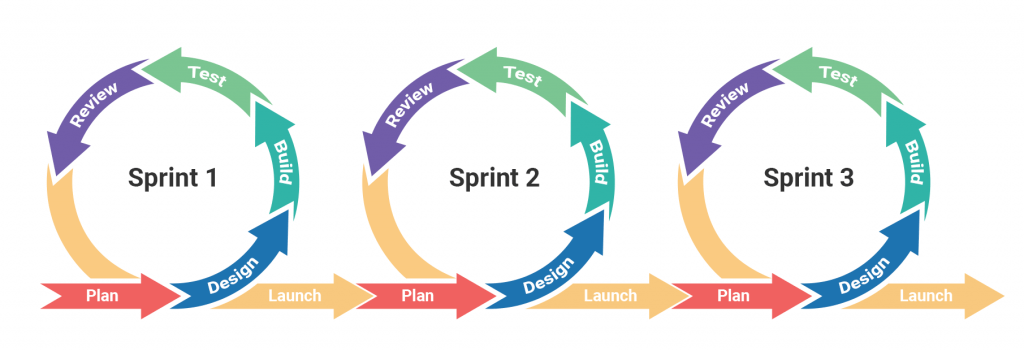
\includegraphics[width=0.8\textwidth]{Figures/agile.png}
    \caption{Modèle de la méthodologie AGILE}
    \label{fig:methodo_agile}
\end{figure}

\section{Planification du projet}

\subsection{Étapes clés}

La planification est une étape clé qui consiste à organiser et prioriser les tâches du projet, à estimer les ressources nécessaires et à identifier les profils requis pour chaque phase. Elle permet également de définir un calendrier réaliste et de répartir les responsabilités au sein de l'équipe. Conformément à la méthodologie adoptée et au contexte de notre projet, nous avons structuré le travail en sprints successifs, chacun ayant des objectifs précis, afin de garantir une livraison itérative, flexible et facilement ajustable en fonction des retours et imprévus.

\begin{itemize}
    \item \textbf{Sprint 0 : Compréhension du projet} \\
    Analyse des besoins et création du backlog produit en priorisant les fonctionnalités de la plateforme de gestion de projets.
    \item \textbf{Sprint 1 : Conception et spécifications techniques} \\
    Modélisation UML (cas d'utilisation, séquences, classes) et définition de l'architecture du système et des interfaces.
    \item \textbf{Sprint 2 : Gestion du paramétrage} \\
    Développement des fonctionnalités de gestion des utilisateurs et des rôles projet.
    \item \textbf{Sprint 3 : Gestion des activités} \\
    Implémentation des modules pour la gestion des projets, sprints, user stories, et tâches.
    \item \textbf{Sprint 4 : Gestion des statistiques} \\
    Création des tableaux de bord et rapports : KPI de projets, vélocité des équipes, burndown charts, et analytics Power BI.
    \item \textbf{Sprint 5 : Tests, validation et déploiement} \\
    Réalisation des tests fonctionnels et d'intégration, correction des anomalies, validation avec les utilisateurs, et déploiement en production.
\end{itemize}

L'approche agile a permis une gestion flexible et réactive, assurant une livraison progressive et cohérente du système. Elle a favorisé une meilleure adaptation aux changements et aux contraintes rencontrées en cours de projet. Grâce aux retours réguliers des utilisateurs, il a été possible d'ajuster les priorités et d'orienter les développements vers les besoins réels. En remplaçant les outils traditionnels comme les diagrammes de Gantt par la planification par sprints, la collaboration au sein de l'équipe a été renforcée, l'efficacité globale améliorée et la visibilité sur l'avancement du projet nettement optimisée.
\subsection{Calendrier prévisionnel et jalons principaux}

% ---- TABLEAU DE PLANIFICATION DES SPRINTS ----

\begingroup
\footnotesize
\setlength{\tabcolsep}{4pt}
\setlength{\LTpre}{12pt}

\begin{longtable}{|p{1.2cm}|p{2.8cm}|p{4.8cm}|p{1.2cm}|p{1.2cm}|p{1.8cm}|p{1.8cm}|}

    \endfirsthead

    \hline
    \textbf{Sprint} & \textbf{TITRE} & \textbf{TÂCHES} & \parbox[t]{1.3cm}{\centering\bfseries PRIO-RITÉ} & \textbf{ÉTAT} & \parbox[t]{1.8cm}{\centering\bfseries DATE DE\\DÉBUT} & \parbox[t]{1.8cm}{\centering\bfseries DATE DE\\FIN} \\
    \hline
    \endhead

\endfoot

    % === CORPS DU TABLEAU (MIS À JOUR POUR LE SYSTÈME DE GESTION DE PROJETS) ===
     % Sprint 00
\multirow{1}{=}{\centering\textbf{Sprint 00}} & \multirow{1}{=}{\centering Étude préliminaire} & Analyse des besoins et création du backlog produit & High & Complete & 01/07/2025 & 06/07/2025 \\ \hline
    % Sprint 01
    \multirow{6}{=}{\centering\textbf{Sprint 01}} & \multirow{6}{=}{\centering Analyse et Conception} & Création des maquettes UI/UX & High & Complete & 07/07/2025 & 10/07/2025 \\ \cline{3-7}
    & & Rédaction du cahier des charges & Normal & Complete & 11/07/2025 & 13/07/2025 \\ \cline{3-7}
    & & Élaboration du diagramme de cas d'utilisation & High & Complete & 14/07/2025 & 16/07/2025 \\ \cline{3-7}
    & & Modélisation du diagramme de classes & Normal & Complete & 17/07/2025 & 19/07/2025 \\ \cline{3-7}
    & & Conception du diagramme de séquence & High & Complete & 20/07/2025 & 22/07/2025 \\ \cline{3-7}
    & & Rédaction du dossier de conception & High & Complete & 23/07/2025 & 25/07/2025 \\ \hline

    % Sprint 02
    \multirow{3}{=}{\centering\textbf{Sprint 02}} & \multirow{3}{=}{\centering Gestion des Utilisateurs} & Développement de l'authentification et autorisation & High & Complete & 26/07/2025 & 28/07/2025 \\ \cline{3-7}
    & & Gestion des rôles et permissions & High & Complete & 29/07/2025 & 31/07/2025 \\ \cline{3-7}
    & & Interface de gestion des utilisateurs & Normal & Complete & 01/08/2025 & 02/08/2025 \\ \hline

    % Sprint 03
    \multirow{4}{=}{\centering\textbf{Sprint 03}} & \multirow{4}{=}{\centering Gestion des Projets} & Création et gestion des projets & High & Complete & 03/08/2025 & 05/08/2025 \\ \cline{3-7}
    & & Gestion des sprints et user stories & High & Complete & 06/08/2025 & 08/08/2025 \\ \cline{3-7}
    & & Système de tâches et Kanban board & High & Complete & 09/08/2025 & 11/08/2025 \\ \cline{3-7}
    & & Gestion des jalons et phases & Normal & Complete & 12/08/2025 & 14/08/2025 \\ \hline

    % Sprint 04
    \multirow{3}{=}{\centering\textbf{Sprint 04}} & \multirow{3}{=}{\centering Tableaux de Bord} & Dashboard principal avec KPI & High & Complete & 15/08/2025 & 16/08/2025 \\ \cline{3-7}
    & & Rapports de vélocité et burndown charts & Normal & Complete & 17/08/2025 & 18/08/2025 \\ \cline{3-7}
    & & Intégration Power BI et analytics & Normal & Complete & 19/08/2025 & 20/08/2025 \\ \hline

    % Sprint 05
    \multirow{2}{=}{\centering\textbf{Sprint 05}} & \multirow{2}{=}{\centering Tests et Livraison} & Tests fonctionnels et vérifications d'intégration & High & Complete & 21/08/2025 & 22/08/2025 \\ \cline{3-7}
& & Livraison finale de la plateforme & Normal & Complete & 23/08/2025 & 25/08/2025 \\ \hline

\caption{Planning des Sprints}
\label{tab:planning_sprints}
\endlastfoot

\end{longtable}
\endgroup

\section{Conclusion}

Ce chapitre a présenté le contexte général et la planification de notre projet de développement d'une plateforme de gestion de projets. Nous avons détaillé la méthodologie Scrum adoptée, le cycle de vie du projet avec ses sept étapes clés, et l'organisation du travail en sprints successifs. Cette approche agile garantit une flexibilité et une adaptabilité optimales face aux évolutions des besoins, tout en maintenant un haut niveau de qualité et une collaboration efficace entre toutes les parties prenantes du projet.